\documentclass[11pt]{article}
\usepackage{preamble}

\begin{document}
  % make title page
\begin{titlepage}
  \newcommand{\HRule}{\rule{\linewidth}{0.5mm}}
  \center
  \textsc{\LARGE Universitetet i Oslo}\\[1.5cm] % Name of your university/college
  \textsc{\Large }\\[0.5cm] % Major heading such as course name
  \textsc{\large FYS3150}\\[0.5cm] % Minor heading such as course title
  \HRule \\[0.4cm]
  { \huge \bfseries Prosjekt 2 }\\[0.4cm] % Title of your document
  \HRule \\[1.5cm]
  \Large \emph{Skrevet av:}\\
  Lyder \textsc{Rumohr Blingsmo} og Bendik \textsc{Samseth}\\[3cm]
  {\large \today}\\[3cm]
  \vfill
\end{titlepage}


\section*{Schödingers likning for to elektroner i en tredimensjonal
  harmonisk oscillator brønn}
\begin{abstract}
  Denne oppgaven skal løse Schödingers likning for to elektroner i en tredimensjonal
  harmonisk oscillator brønn med og uten en
  Coulomb-vekselvirkning. For å gjøre dette blir likningen skrevet om
  til diskret form som en eigenverdilikning. Denne blir så løst ved
  hjelp av en implementasjon av Jacobis metode. 
\end{abstract}

\section{Omskrivning av problemet}

\subsection{Static Coulomb interaction}
Vi antar at to elektroner befinner seg i et tredimensjonalt harmonisk
oscillator (HO) brønnpotensial, og at de vekselvirker gjennom
Coulombpotensialet mellom dem. Vi antar sfærisk symmetri. 

Vi er først interessert i løsningen på den radielle delen av
Schödingers likning (SL) for et elektron. Denne likningen kan skrives
som 
\begin{align}
  -\frac{ \hbar^2 }{ 2m }\left( \frac{ 1 }{ r^2 }\frac{ d }{ dr }r^2
  \frac{ d }{ dr } - \frac{ l(l+1) }{ r^2 }   \right) R(r) + V(r)R(r)
  = ER(r).\label{eq:SL}
\end{align}
I dette tilfellet har vi et HO-potensial $(1/2)kr^2$ med $k=m\omega^2$
og $E$ er energien til oscillatoren i tre dimensjoner. $\omega$ kalles
oscillatorfrekvensen. Energien er gitt som 
\begin{align}
  E_{nl} = \hbar\omega\left(2n+l+\frac{ 3 }{ 2 }\right)\label{eq:Energy}
\end{align}
med $n=1,2,\dots$ og $l=0,1,2,\dots$. Fordi vi har sfæriske
koordinater har vi $r\in [0,\infty)$. $l$ representerer elektronets
angulærmoment. 

Vi begynner omskrivningen med å substituere $R(r) = u(r)/r$ og får 
\begin{align*}
  -\frac{ \hbar^2 }{ 2m }\frac{ d^2 }{ dr^2 }u(r) + \left(V(r) +
  \frac{ l(l+1) }{ r^2 }\frac{ \hbar^2 }{ 2m }\right)u(r) = Eu(r).
\end{align*}
Grensebetingelsene blir nå $u(0)=0$ og $u(\infty)=0$. 

Vi gjennomfører nok en substitusjon ved å definere $\rho = r/\alpha$,
der $\alpha$ er en konstant med dimensjon lengde. Vi får:
\begin{align*}
  -\frac{ \hbar^2 }{ 2m\alpha^2 }\frac{ d^2 }{ d\rho^2 }u(\rho) +
  \left(V(\rho) + \frac{ l(l+1) }{ \rho^2 }\frac{ \hbar^2 }{
  2m\alpha^2 }\right)u(\rho) = Eu(\rho).
\end{align*}

I denne oppgaven setter vi $l=0$, dvs. at elektronet ikke har
angulærmoment. Nå kan vi sette inn potensialet $V(\rho) =
(1/2)k\alpha^2\rho^2$, og vi ender med følgende likning:
\begin{align*}
   -\frac{ \hbar^2 }{ 2m\alpha^2 }\frac{ d^2 }{ d\rho^2 }u(\rho) +
  \left( \frac{ k }{ 2 }\alpha^2\rho^2u(\rho) \right)u(\rho) = Eu(\rho).
\end{align*}
Deler vi så med faktoren i første ledd får vi
\begin{align*}
    \frac{ d^2 }{ d\rho^2 }u(\rho) + \frac{ mk }{ \hbar^2
  }\alpha^4\rho^2u(\rho) u(\rho) = \frac{ 2m\alpha^2 }{ \hbar^2 }Eu(\rho).
\end{align*}

$\alpha$ er en konstant vi har valgt, så den kan vi nå bestemme slik
at 
\begin{align*}
  \frac{ mk }{ \hbar^2 }\alpha^4 = 1 \Leftrightarrow \alpha = \left(\frac{ \hbar^2 }{ mk }\right)^{1/4}.
\end{align*}
Definerer vi til slutt $\lambda$ ved
\begin{align*}
  \lambda = \frac{ 2m\alpha^2 }{ \hbar^2 }E,
\end{align*}
så kan vi omskrive \eqref{eq:SL} som
\begin{align}
  -\frac{ d^2 }{ d\rho^2 }u(\rho) + \rho^2u(\rho) = \lambda u(\rho).\label{eq:SL-rewrite}
\end{align}
Dette er den første likningen som skal løses numerisk.





\subsection{Repulsive Coulomb interaction}

We will now study two electrons in a harmonic oscillator well which
also interact via a repulsive Coulomb interaction.
Let us start with the single-electron equation written as
\[
  -\frac{\hbar^2}{2 m} \frac{d^2}{dr^2} u(r) 
       + \frac{1}{2}k r^2u(r)  = E^{(1)} u(r),
\]
where $E^{(1)}$ stands for the energy with one electron only.
For two electrons with no repulsive Coulomb interaction, we have the following 
Schr\"odinger equation
\[
\left(  -\frac{\hbar^2}{2 m} \frac{d^2}{dr_1^2} -\frac{\hbar^2}{2 m} \frac{d^2}{dr_2^2}+ \frac{1}{2}k r_1^2+ \frac{1}{2}k r_2^2\right)u(r_1,r_2)  = E^{(2)} u(r_1,r_2) .
\]


Note that we deal with a two-electron wave function $u(r_1,r_2)$ and 
two-electron energy $E^{(2)}$.

With no interaction this can be written out as the product of two
single-electron wave functions, that is we have a solution on closed form.

We introduce the relative coordinate ${\bf r} = {\bf r}_1-{\bf r}_2$
and the center-of-mass coordinate ${\bf R} = 1/2({\bf r}_1+{\bf r}_2)$.
With these new coordinates, the radial Schr\"odinger equation reads
\[
\left(  -\frac{\hbar^2}{m} \frac{d^2}{dr^2} -\frac{\hbar^2}{4 m} \frac{d^2}{dR^2}+ \frac{1}{4} k r^2+  kR^2\right)u(r,R)  = E^{(2)} u(r,R).
\]

The equations for $r$ and $R$ can be separated via the ansatz for the 
wave function $u(r,R) = \psi(r)\phi(R)$ and the energy is given by the sum
of the relative energy $E_r$ and the center-of-mass energy $E_R$, that
is
\[
E^{(2)}=E_r+E_R.
\]

We add then the repulsive Coulomb interaction between two electrons,
namely a term 
\[
V(r_1,r_2) = \frac{\beta e^2}{|{\bf r}_1-{\bf r}_2|}=\frac{\beta e^2}{r},
\]
with $\beta e^2=1.44$ eVnm.

Adding this term, the $r$-dependent Schr\"odinger equation becomes
\[
\left(  -\frac{\hbar^2}{m} \frac{d^2}{dr^2}+ \frac{1}{4}k r^2+\frac{\beta e^2}{r}\right)\psi(r)  = E_r \psi(r).
\]
This equation is similar to the one we had previously in (a) and we introduce
again a dimensionless variable $\rho = r/\alpha$. Repeating the same
steps as in (a), we arrive at 
\[
  -\frac{d^2}{d\rho^2} \psi(\rho) 
       + \frac{1}{4}\frac{mk}{\hbar^2} \alpha^4\rho^2\psi(\rho)+\frac{m\alpha \beta e^2}{\rho\hbar^2}\psi(\rho)  = 
\frac{m\alpha^2}{\hbar^2}E_r \psi(\rho) .
\]
We want to manipulate this equation further to make it as similar to that in (a)
as possible. We define a 'frequency' 
\[
\omega_r^2=\frac{1}{4}\frac{mk}{\hbar^2} \alpha^4,
\]
and fix the constant $\alpha$ by requiring 
\[
\frac{m\alpha \beta e^2}{\hbar^2}=1
\]
or 
\[
\alpha = \frac{\hbar^2}{m\beta e^2}.
\]
Defining 
\[
\lambda = \frac{m\alpha^2}{\hbar^2}E,
\]
we can rewrite Schr\"odinger's equation as
\[
  -\frac{d^2}{d\rho^2} \psi(\rho) + \omega_r^2\rho^2\psi(\rho) +\frac{1}{\rho} = \lambda \psi(\rho).
\]
We treat $\omega_r$ as a parameter which reflects the strength of the oscillator potential.

Here we will study the cases $\omega_r = 0.01$, $\omega_r = 0.5$, $\omega_r =1$,
and $\omega_r = 5$   
for the ground state only, that is the lowest-lying state.





\section{Diskretisering}
Vi skal nå få likning \eqref{eq:SL-rewrite} over på en diskret
form. Til dette bruker vi det vanlige uttrykket for den andrederiverte
av en funksjon $u$, 
\begin{align*}
  u'' = \frac{ u(\rho + h) - 2u(\rho) + u(\rho-h) }{ h^2 } + \mathcal{O}(h^2)
\end{align*}
der $h$ er steglengden vi bruker. Vi må også bestemme en minimum- og
maksimumverdi for $\rho$. Vi har egentlig $\rho\in [0,\infty)$, men vi
kan åpenbart ikke ha $\infty$ som en verdi. Vi setter dermed
$\rho_{min} = 0$ og $\rho_{maks}$ som en gitt verdi. Vi burde passe på
at valget av $\rho_{maks}$ ikke ødelegger resultatet vårt ved å prøve
flere mulige verdier. 

Hvis vi ønsker et gitt antall steg, $n_{step}$ så definerer vi $h$ som
\begin{align*}
  h = \frac{ \rho_{maks} - \rho_{min} }{ n_{step} }.
\end{align*}
Da er $\rho_i$ gitt ved
\begin{align*}
  \rho_i = \rho_{min} + ih\hspace{1cm} i=0,1,2,\dots,n_{step}.
\end{align*}
Videre innfører vi $u_{i\pm 1} = u(\rho_i \pm h)$, og $V_i =
\rho_i^2$. Da kan vi skrive likning \eqref{eq:SL-rewrite} på
følgende vis:
\begin{align*}
  -\frac{ u_{i+1} - 2u_i + u_{i-1} }{ h^2 } + V_iu_i = \lambda u_i.
\end{align*}

Fra denne likningen setter vi de diagonale matriseelementene som 
\begin{align*}
  d_i = \frac{ 2 }{ h^2 } + V_i,
\end{align*}
og de ikke-diagonale matriseelementene blir 
\begin{align*}
  e_i = -\frac{ 1 }{ h^2 }.
\end{align*}
Vi merker oss at alle $e_i$ er like. Med disse definisjonene tar SL
følgende form:
\begin{align*}
  d_iu_i + e_{i-1}u_{i_1} + e_{i+1}u_{i+1} = \lambda u_i.
\end{align*}
der $u_i$ er ukjent. Denne likningen kan skrives på matriseform som
en eigenverdilikning,
\begin{align}
  \left(\begin{array}{ccccccc}
      d1 & e_1 & 0 & 0 & \dots & 0 & 0\\
      e_1& d_2 & e_2 & 0 & \dots & 0 & 0\\
      0  & e_2 & d_3 & e_3 & 0 & \dots & 0\\
      \dots & \dots & \dots & \dots & \dots & \dots & \dots\\
      0 & \dots & \dots & \dots & \dots & d_{n_{step}-2} & e_{n_{step}-1}\\
      0 & \dots & \dots & \dots & \dots & e_{n_{step}-1} & d_{n_{step}-1}
    \end{array}\right)
    \left(\begin{array}{c}
        u_1\\
        u_2\\
        \dots\\
        \dots\\
        \dots\\
        u_{n_{step}-1}
      \end{array}\right) = 
     \lambda 
    \left(\begin{array}{c}
        u_1\\
        u_2\\
        \dots\\
        \dots\\
        \dots\\
        u_{n_{step}-1}
      \end{array}\right)\label{eq:SL-matrix}.
\end{align}

\section{Implementasjon av Jacobis rotasjons-algoritme}
For å løse egenverdiligningen har vi brukt Jacobis rotasjons-algoritme. 
Hovedideen er å gjøre gjentatte similærtransformasjoner(med en rotasjonsmatrise) av 
matrisen inntil matrisen er tilstrekkelig diagonal. Vi sier at den er diagonal nok, når største 
ikke-diagonale matriseelement er under en gitt toleranse,  $ max(A_{ij}) < \epsilon$. Algoritmen er gitt
i forelesningsnotatene~\cite[seksjon 7.4, side 215]{Lecture-notes}. Vår implementasjon kan sees på github-repo \footnote{\url{https://github.com/bsamseth/fys3150-project2.git}}


Vi definerer $\tan\theta = t= s/c$, med $s=\sin\theta$ og $c=\cos\theta$ og
\[\cot 2\theta=\tau = \frac{a_{ll}-a_{kk}}{2a_{kl}}.
\]
For hver similærtransformasjon ønsker vi å velge $\theta$ slik at to ikke-diagonale matriseelementer blir 0. 
 Vi får andregradsligningen(bruker $\cot 2\theta=1/2(\cot \theta-\tan\theta)$
\[
t^2+2\tau t-1= 0,
\]
som gir 
\[
  t = -\tau \pm \sqrt{1+\tau^2},
\]
og $c$ og $s$ får vi lett fra
\[
   c = \frac{1}{\sqrt{1+t^2}},
\]
og $s=tc$. 

Men for hver similærtransformasjon endres også noen andre elementer i matrisen. For 
å minimere forskjellen, og forsikre oss om at matrisen blir stadig mer diagonal, 
velger $t$ til å være den minste av røttene. Dette forsikrer oss om at $|\theta| \le \pi/4$ \ref{fig:theta} og minimerer derfor differansen mellom ${\bf B}$ og ${\bf A}$ siden
\[
||{\bf B}-{\bf A}||_F^2=4(1-c)\sum_{i=1,i\ne k,l}^n(a_{ik}^2+a_{il}^2) +\frac{2a_{kl}^2}{c^2}.
\]
siden små $\theta$ gir små $c$.

\begin{figure}[ht]
  \centering
  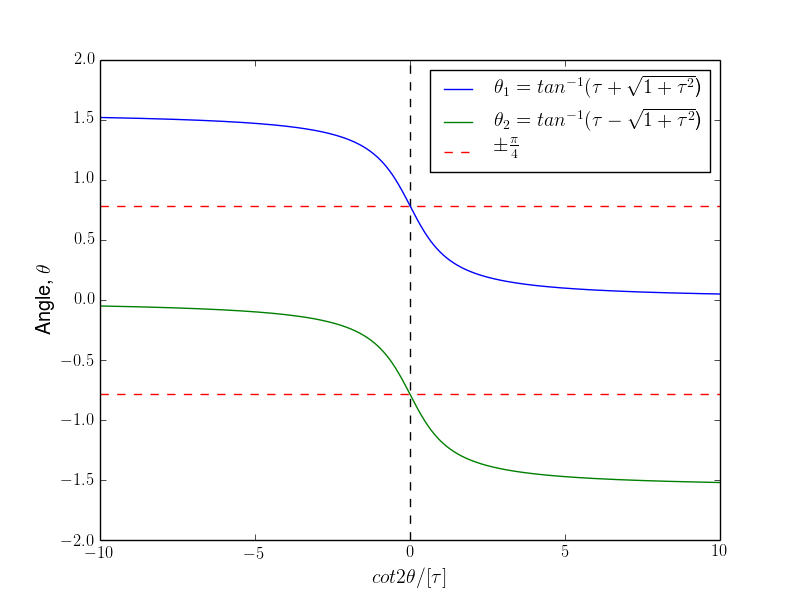
\includegraphics[scale=0.7]{theta.png}
  \caption{\label{fig:theta} For hver $\tau$ får vi to muligheter for $\theta$. Fra plottet ser vi at vi alltid kan velge enten $\theta_1$ eller $\theta_2$ slik at $|\theta| \le \pi/4$ }
\end{figure}

\subsection{Test av algoritmen}

\section{Resultater}







\printbibliography
\end{document}
%%% Local Variables:
%%% mode: latex
%%% TeX-master: t
%%% End:
